\documentclass[aspectratio=169]{beamer}

\input{ceesd-macros.tex}

\newif\ifmovies
\moviestrue
%\moviesfalse

\newif\ifsubs
\substrue
%\subsfalse

\newif\ifnotes
\notestrue
% \notesfalse

% AK Additions
\usetikzlibrary{fit}
\usetikzlibrary{shadows}
\usetikzlibrary{positioning}
\usetikzlibrary{shapes.arrows}
\def\evalprint#1{{\pgfmathtruncatemacro{\mathresult}{#1}\mathresult}}
\def\credit#1{{\scriptsize[#1]}}
\let\b=\boldsymbol
\setbeamercolor{alerted text}{fg=IllinoisOrange}
\usepackage{listings}
\definecolor{codegreen}{rgb}{0,0.6,0}
\definecolor{codegray}{rgb}{0.5,0.5,0.5}
\definecolor{codepurple}{rgb}{0.58,0,0.82}
\definecolor{backcolour}{rgb}{0.95,0.95,0.92}
\lstdefinestyle{akcodestyle}{
    basicstyle=\small,
    backgroundcolor=\color{gray!20},
    commentstyle=\color{codegreen},
    keywordstyle=\color{magenta},
    numberstyle=\tiny\color{codegray},
    stringstyle=\color{codepurple},
    basicstyle=\ttfamily\footnotesize,
    columns=flexible
}
\def\didit#1{\prj{\tiny}{#1}}
\def\software#1{\textit{#1}}
\def\good#1{\textcolor{green!50!black}{#1}}
\def\okay#1{\textcolor{green!25!gray}{#1}}
\def\notideal#1{\textcolor{IllinoisOrange}{#1}}
\def\bad#1{\textcolor{red}{#1}}
\def\future{\textcolor{blue}{Future work:}}
\def\progress#1{\okay{In Progress:}}
\def\draft#1{\okay{Draft Available:}}
\def\completed{\good{Completed:}}
% End AK Additions

\begin{document}



%======================================================================
\begin{frame}\frametitle{}

\vspace*{0.2in}

\hspace*{0.0in}\textrm{{\huge\bfseries\color{myOrange} NCSA-WEST: NCSA-Workshop on Exascale Simulation Technologies}}

\vspace*{0.2in}
\hrule
\begin{center}
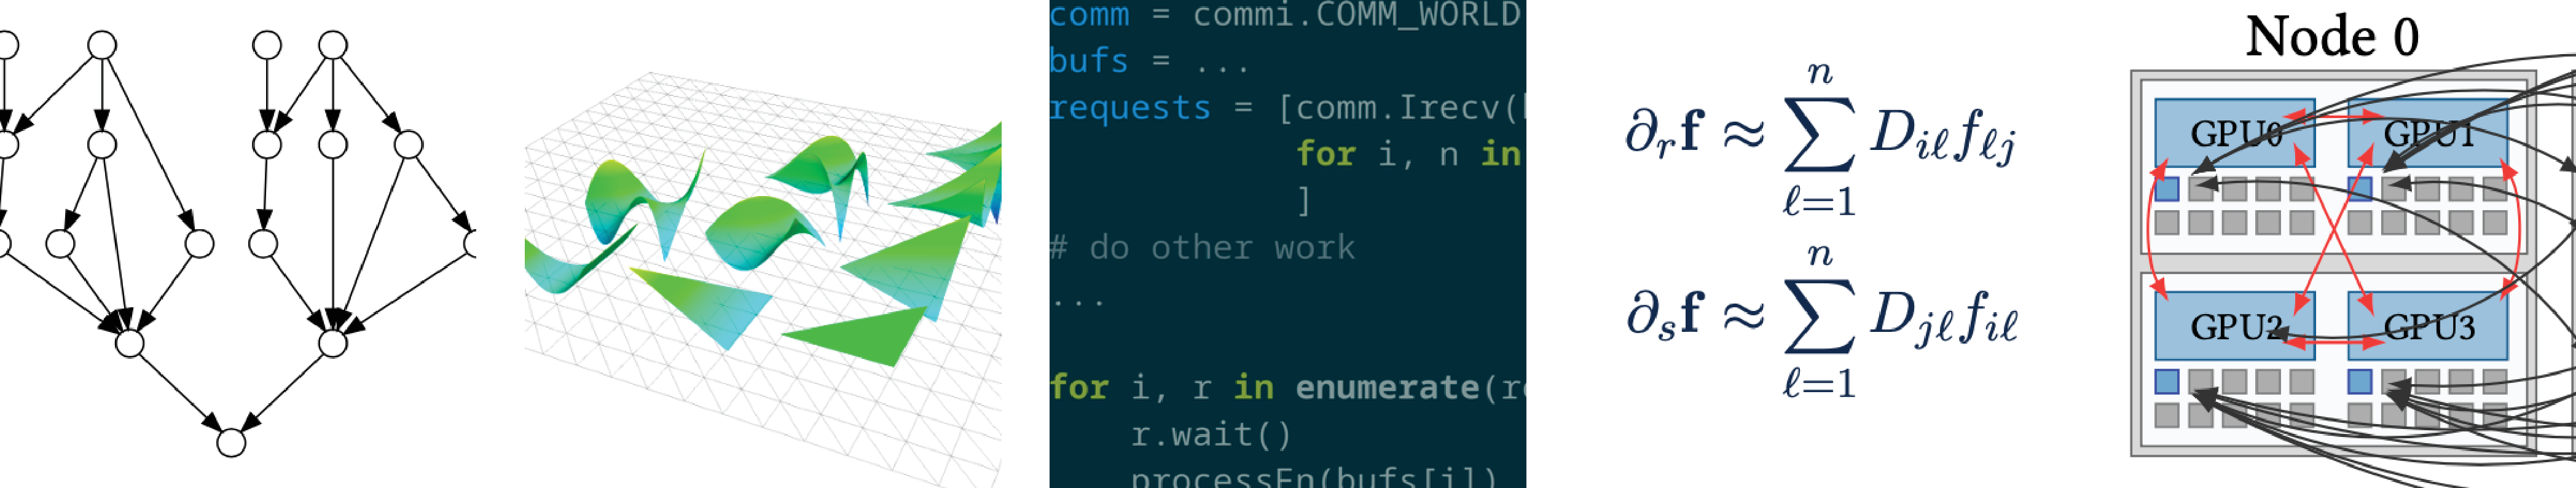
\includegraphics[width=0.75\textwidth]{coverart-cs.pdf}
\end{center}
\hrule

\vspace*{0.1in}
\ \hbox{}\hfill\cPI{Luke Olson} \rPI{(CS)}\\
\ \hbox{}\hfill\cPI{Jonathan Freund} \rPI{(AE)}\\
\ \hbox{}\hfill\cPI{Bill Gropp} \rPI{(CS/NCSA)}\\
\ \hbox{}\hfill\cPI{Andreas Kl\"ockner} \rPI{(CS)}\\
\ \hbox{}\hfill\cPI{Daniel S. Katz} \rPI{(NCSA)}\\

\end{frame}

% A little about us
% [3] What led to the workshop
%    - (red) June workshop on PSAAP, proposed NUWEST
%        - highlight goals
%    - --> (orange) Roadtest the tools (MIRGE/Parsl) and the format
%    - (yellow) Revise based on your input
%    - (green) NUWEST, January 2024
% [1] PSAAP: predictive science program
% [2] CEESD overview
% [3] What led to the workshop
%    - (red) June workshop on PSAAP, proposed NUWEST
%        - highlight goals
%    - --> (orange) Roadtest the tools (MIRGE/Parsl) and the format
%    - (yellow) Revise based on your input
%    - (green) NUWEST, January 2024
% [4] Center MIRGE
% [5] Format
% [6] Follow up
\begin{frame}{What is this workshop about?}
\begin{center}
Goal: To highlight key technologies for facilitating exascale predictive science
\end{center}
\begin{itemize}
\item Showcase and characterize technologies in CEESD
\item Identify challenges and limitations
\item Provide opportunities to initiate collaboration at NCSA and beyond
\end{itemize}
\end{frame}

\begin{frame}{Predictive Science Academic Alliance Program (PSAAP)}
\url{psaap.llnl.gov}
      \begin{itemize}
        \item \ldots to further predictive science enabled by effective Exascale computing technologies;
        \item \ldots technologies to support effective exascale computing in science/engineering; and
        \item Predictive science \ldots for large-scale simulations
      \end{itemize}
  \begin{center}
    \tiny
    \begin{tabular}{m{1cm}m{4cm}m{8cm}}
      \includegraphics[width=.5cm]{./figures/logo_cu.png}&
      University of Colorado at Boulder& Center for Micromorphic Multiphysics Porous and Particulate Materials Simulations with Exascale Computing Workflows\\
      \includegraphics[width=.5cm]{./figures/logo_ceesd.png}&
      University of Illinois& Center for Exascale-Enabled Scramjet Design\\
      \includegraphics[width=.5cm]{./figures/logo_ut.png}&
      University of Texas at Austin& Exascale Predictive Simulation of Inductively Coupled Plasma Torches\\
      \includegraphics[width=.5cm]{./figures/logo_stanford.png}&
      Stanford University& Integrated Simulations using Exascale Multiphysics Ensembles\\
      \includegraphics[width=.5cm]{./figures/logo_buffalo.png}&
      University at Buffalo& Center for Exascale Simulation of Hybrid Rocket Motors\\
      \includegraphics[width=.5cm]{./figures/logo_mit.png}&
      Massachusetts Institute of Technology& Center for the Exascale Simulation of Material Interfaces in Extreme Environments\\
      \includegraphics[width=.5cm]{./figures/logo_maryland.png}&
      University of Maryland& Solution-Verification, Grid-Adaption and Uncertainty Quantification for Chaotic Turbulent Flow Problems\\
      \includegraphics[width=.5cm]{./figures/logo_unm.png}&
      University of New Mexico& Center for Understandable, Performant Exascale Communication\\
      \includegraphics[width=.5cm]{./figures/logo_osu.png}&
      Oregon State University& Center for Exascale Monte Carlo Neutron Transport
    \end{tabular}
  \end{center}
\end{frame}

\begin{frame}{CEESD:  The Center for Exascale-enabled Scramjet Design}
\begin{itemize}
\item \sPI{scramjet} --- \underline{the} technology for air-breathing
  hypersonics propulsion

\item Employ light-weight, high-$T$ composite materials to advance designs

\begin{center}
\begin{minipage}{0.45\textwidth}
\includegraphics[width=\textwidth]{figures/scramjet-LaRC.png}
\end{minipage}
\hfil
\begin{minipage}{0.45\textwidth}
\raisebox{0.3in}{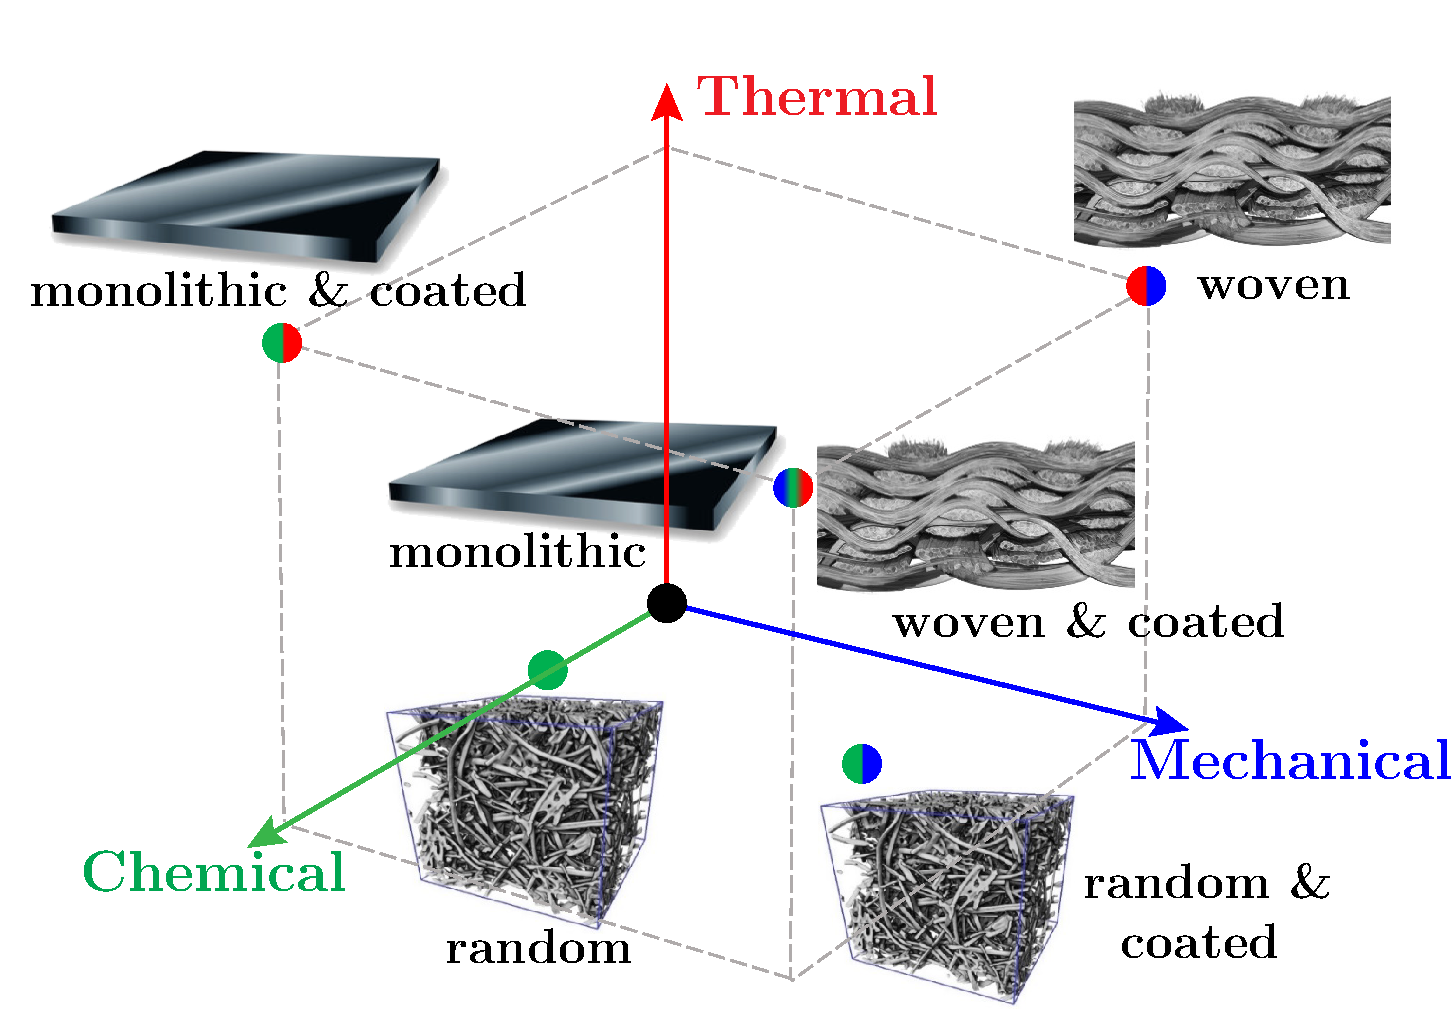
\includegraphics[width=\textwidth]{figures/composite-design.pdf}}
\end{minipage}
\end{center}

  \item \rPI{Predictive confidence}:  avoid costly/prohibitive testing,
    accelerate design and innovation
\end{itemize}
\end{frame}

\begin{frame}\frametitle{CEESD simulations}

  % \centerline{\cPI{\Large Usability --- portability --- performance}}

\medskip
    \begin{itemize}
    \item \rPI{Usability}:

      \noindent Python-based simulation (performance with MIRGE)

      \noindent Python-based workflows (ease of execution with Parsl)
    \end{itemize}
  \bigskip

  \begin{itemize}
  \item \rPI{Portability}:  Runs ``out of the box''  on most systems:  performance with MIRGE, execution and job submission enhanced by Parsl
  \end{itemize}
    \vspace*{-0.1in}
    \begin{center}
      \begin{tabular}{ccccc}
        \includegraphics[width=0.15\textwidth]{figures/comp-mac.png}
        &
          \includegraphics[width=0.1505\textwidth]{figures/comp-quartz.png}
        &
          \includegraphics[width=0.16\textwidth]{figures/comp-lassen.png}
        &
          \includegraphics[width=0.1505\textwidth]{figures/comp-delta.png}&
        \raisebox{0.2in}{\cPI{$\cdots$}}\\
        \cPI{Mac/Linux} & \cPI{LLNL--Quartz} &
                                                       \cPI{LLNL-Lassen}
        &\cPI{NCSA-Delta} & \\
        \rPI{laptop/workstn.} & \rPI{multi-core/node} &
                                                       \rPI{4GPU/node}
        & \rPI{4GPU/node} & \\
        \rPI{\footnotesize AMD, Intel, M1, M2} \\
      \end{tabular}
    \end{center}


\end{frame}

\begin{frame}{Exascale Technologies}
  \begin{center}
    \fbox{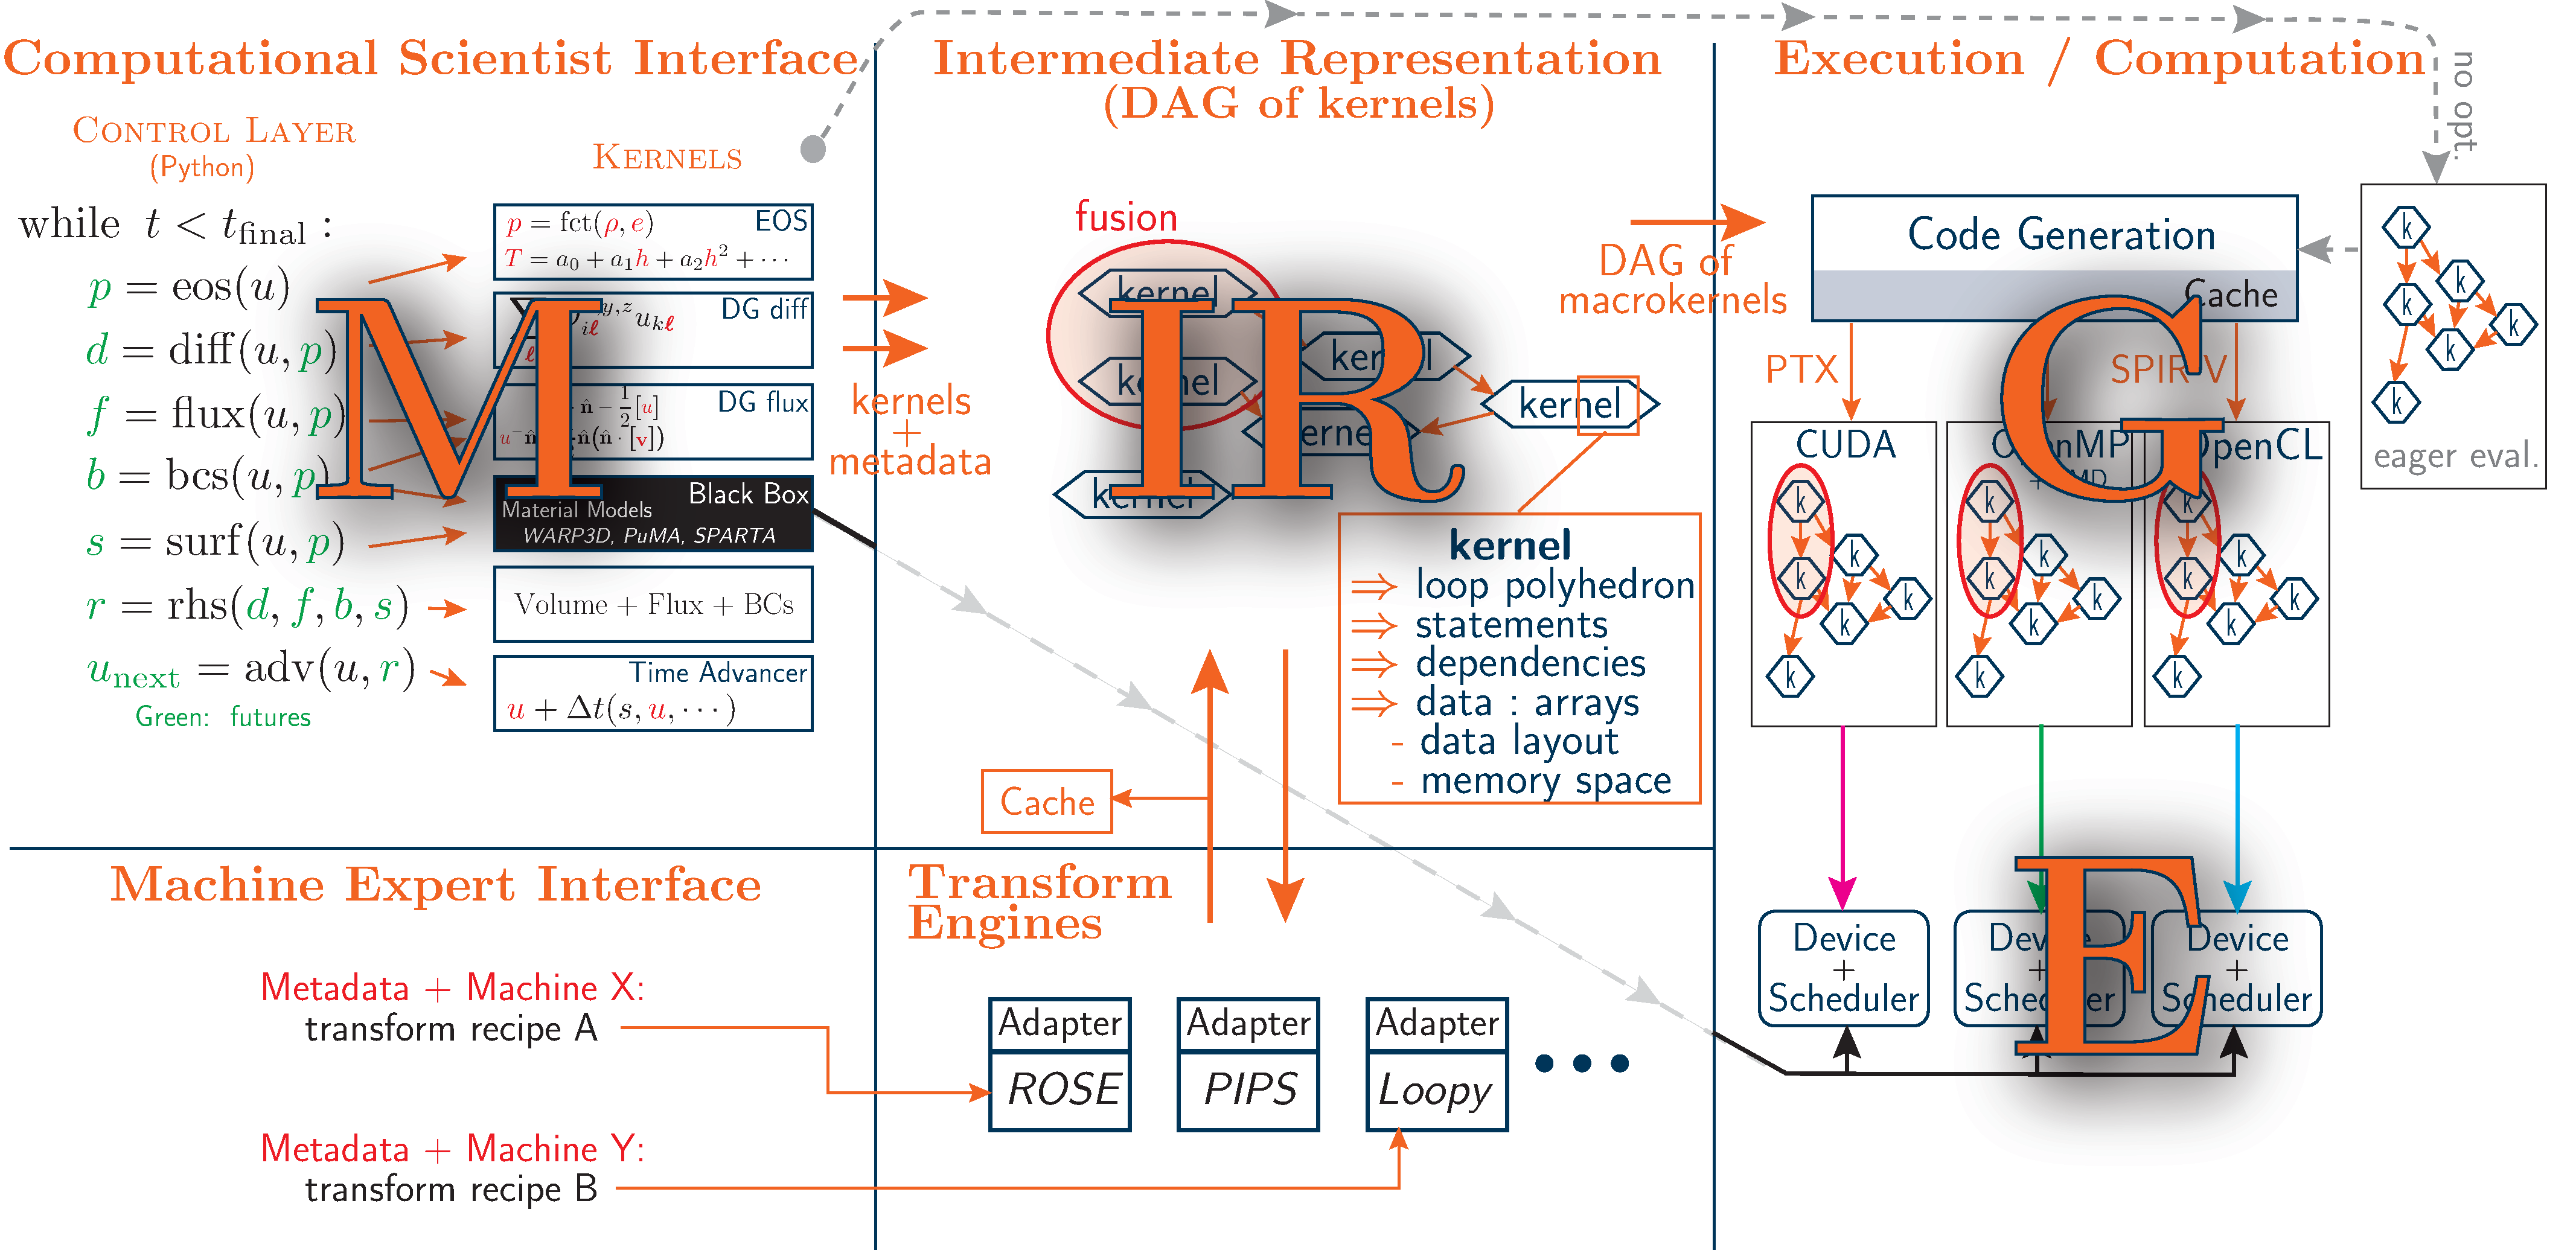
\includegraphics[width=3cm]{figures/controllayerMIRGE-new.pdf}}
    \hspace{1cm}
    \fbox{\includegraphics[width=3cm]{./figures/parsl.png}}
    \hspace{1cm}
    \fbox{\includegraphics[width=3cm]{./figures/funcx.png}}
  \end{center}

  Center has utilized on and accelerated two key exascale tools:
\begin{itemize}
\item MIRGE:
    \cPI{M}ath $\cdot$
    \cPI{I}ntermediate \cPI{R}epresentation $\cdot$
    \cPI{G}eneration $\cdot$
    \cPI{E}xecution
  \begin{itemize}
  \item \emph{Idea:} Tensorflow for HPC/immutable arrays for everything
  \item \emph{Scientist interface:} arrays, array contexts, array containers
  \item \emph{Intermediate Representations:} Array data flow graph, loop IR
  \item \emph{Transform path:} metadata, metadata propagation, writing transforms
  \end{itemize}
\item Parsl:
\begin{itemize}
\item \emph{Idea:} Workflows as asynchronous Python code
\item \emph{Predictive Science Applications:} Remote runs, pre-/postprocessing, UQ sampling
\item \emph{Implementation:} `Macro' graph of dependencies, scheduling, funcX, Globus
\end{itemize}
\end{itemize}
\end{frame}

\begin{frame}[fragile=singleslide]{Format}

  \begin{itemize}
    \item Short (short!) overview on the MIRGE/Parsl vision
    \item Hands-on demos.
  \end{itemize}
  \begin{verbatim}
 900– 915: Brief Introduction, overview (Olson)
 915- 930: MIRGE: conceptual overview   (Klöckner)
 930–1000: MIRGE: hands-on example
1000-1015: break
1015-1030: Parsl: conceptual overview   (Katz, D. Friedel)
1030–1100: Parsl: hands-on example
1100-1200: Bring your own code
  \end{verbatim}


  \bigskip
  \cPI{We want your feedback!}  What went well, what can be improved.
\end{frame}


%======================================================================
\begin{frame}\frametitle{}

\vspace*{0.2in}

\begin{center}

\includegraphics[width=0.35\textwidth]{ceesd-logo-2.pdf}

\vspace*{0.35in}
\cPI{\huge Questions?}

\vspace*{0.5in}
\begin{minipage}{0.6\textwidth}
This material is based in part upon work supported by the Department of Energy, National Nuclear Security Administration, under Award Number DE-NA0003963. 
\end{minipage}



\end{center}


\end{frame}
%======================================================================


\end{document}
